\documentclass{article}
\usepackage[margin=1in]{geometry}
\usepackage{amsmath}
\usepackage{amssymb}
\usepackage{booktabs}
\usepackage{tikz}
\usetikzlibrary{positioning, arrows.meta, shapes.geometric, calc, decorations.pathreplacing}

\begin{document}

\title{Disturbance Rejection Capability:\\Maximum Allowable Speed Analysis}
\author{}
\date{}
\maketitle

% =============================================================================
\section{Understanding the Control System}
% =============================================================================

\subsection{What is the ``Disturbance''?}

In this radar system, the target motion causes a Doppler phase shift, which is treated as the disturbance that the controller must cancel.

% TikZ: Disturbance Concept Box
\begin{figure}[h]
\centering
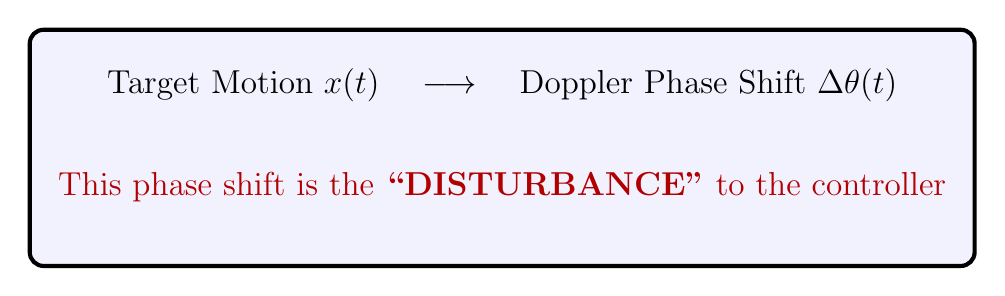
\begin{tikzpicture}[
    box/.style={rectangle, draw=black, line width=1.5pt, rounded corners=5pt, 
                minimum width=12cm, minimum height=3cm, fill=blue!5},
    arrow/.style={-{Stealth[length=4mm, width=3mm]}, line width=1.5pt}
]
    % Main box
    \node[box] (main) at (0,0) {};
    
    % Content
    \node[font=\large] at (0, 0.8) {Target Motion $x(t)$ \quad $\longrightarrow$ \quad Doppler Phase Shift $\Delta\theta(t)$};
    \node[font=\large, text=red!70!black] at (0, -0.5) {This phase shift is the \textbf{``DISTURBANCE''} to the controller};
    
\end{tikzpicture}
\caption{The disturbance in the radar control system.}
\end{figure}

The Doppler phase shift is given by:
\begin{equation}
\Delta\theta(t) = \frac{4\pi}{\lambda} x(t)
\end{equation}

% =============================================================================
\subsection{What Does the Controller Do?}

\textbf{Goal:} Keep $\theta = \pi$ (the desired operating point)

% TikZ: Control System Block Diagram
\begin{figure}[h]
\centering
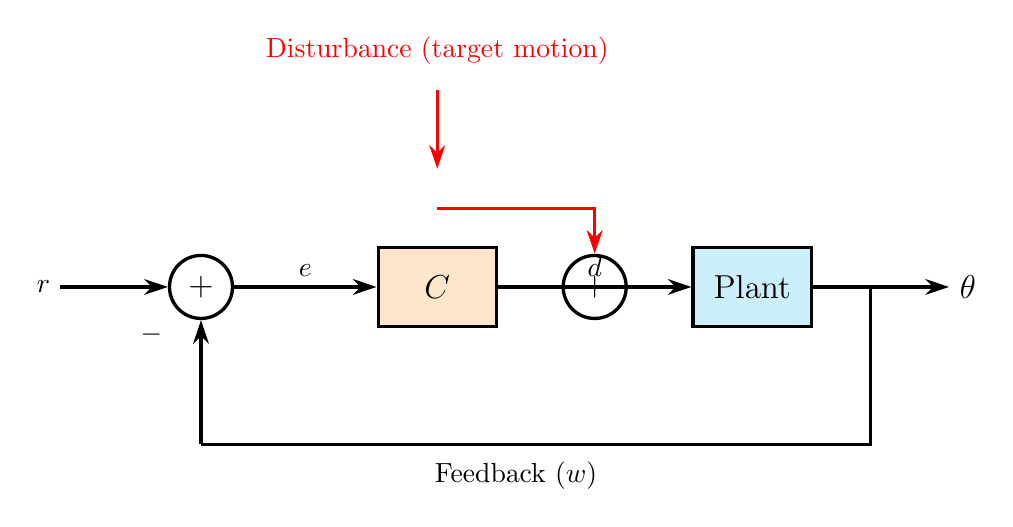
\begin{tikzpicture}[
    block/.style={rectangle, draw=black, line width=1.2pt, minimum width=1.5cm, 
                  minimum height=1cm, font=\large},
    sum/.style={circle, draw=black, line width=1.2pt, minimum size=0.8cm, font=\large},
    arrow/.style={-{Stealth[length=3mm, width=2mm]}, line width=1.2pt},
    label/.style={font=\normalsize}
]

    % Disturbance arrow
    \node[font=\normalsize, text=red] at (3, 3) {Disturbance (target motion)};
    \draw[arrow, red] (3, 2.5) -- (3, 1.5);
    
    % Sum block
    \node[sum] (sum) at (0, 0) {$+$};
    \node[label, below left=0.1cm of sum] {$-$};
    
    % Controller
    \node[block, fill=orange!20] (ctrl) at (3, 0) {$C$};
    
    % Plant
    \node[block, fill=cyan!20] (plant) at (7, 0) {Plant};
    
    % Input
    \node[label] (r) at (-2, 0) {$r$};
    \draw[arrow] (r) -- (sum);
    
    % Sum to Controller
    \draw[arrow] (sum) -- (ctrl) node[midway, above] {$e$};
    
    % Controller to Plant
    \draw[arrow] (ctrl) -- (plant) node[midway, above] {$d$};
    
    % Output
    \draw[arrow] (plant) -- ++(2.5, 0) node[right, font=\large] {$\theta$};
    
    % Feedback
    \draw[line width=1.2pt] (8.5, 0) -- (8.5, -2) -- (0, -2);
    \draw[arrow] (0, -2) -- (sum);
    \node[label] at (4, -2.4) {Feedback ($w$)};
    
    % Disturbance input to sum before plant
    \node[sum] (sum2) at (5, 0) {$+$};
    \draw[arrow, red] (3, 1) -- (5, 1) -- (sum2);
    
\end{tikzpicture}
\caption{Control system block diagram with disturbance.}
\end{figure}

\begin{itemize}
    \item $r = 0$: Set-point (desired frequency shift = 0, meaning $\theta = \pi$)
    \item \textbf{Disturbance}: Doppler phase shift from target motion
    \item \textbf{Controller output} $d$: Tunable delay that cancels the disturbance
\end{itemize}

% =============================================================================
\section{Why Maximum Speed = Disturbance Rejection?}
% =============================================================================

\subsection{The Faster the Target Moves $\rightarrow$ The Larger the Disturbance Rate}

\begin{table}[h]
\centering
\renewcommand{\arraystretch}{1.5}
\begin{tabular}{lcc}
\toprule
\textbf{Target Speed} & \textbf{Phase Change Rate} & \textbf{Controller Difficulty} \\
\midrule
Slow & Small $\frac{d\theta}{dt}$ & Easy to track \\
Fast & Large $\frac{d\theta}{dt}$ & Hard to track \\
Too Fast & Controller can't keep up & \textcolor{red}{\textbf{Loses lock!}} \\
\bottomrule
\end{tabular}
\caption{Relationship between target speed and controller difficulty.}
\end{table}

\subsection{Mathematical Relationship}

Target moving at constant speed $v$:
\begin{equation}
x(t) = v \cdot t
\end{equation}

Phase shift:
\begin{equation}
\Delta\theta(t) = \frac{4\pi}{\lambda} \cdot v \cdot t = \frac{2\omega_n}{c} \cdot v \cdot t
\end{equation}

\textbf{Rate of phase change:}
\begin{equation}
\frac{d(\Delta\theta)}{dt} = \frac{2\omega_n \cdot v}{c}
\end{equation}

The faster the target ($v \uparrow$), the faster the phase changes, and the harder it is for the controller to cancel!

% =============================================================================
\section{Phase Error Analysis}
% =============================================================================

\subsection{What Happens When Controller Can't Keep Up?}

The controller tries to regulate $\theta$ to $\pi$, but has limited bandwidth $\omega_{BW}$.

\textbf{Phase error} $e = \theta - \pi$ accumulates when:
\begin{equation}
\text{Disturbance rate} > \text{Controller bandwidth}
\end{equation}

\subsection{Steady-State Phase Error}

From the paper (equation 17):
\begin{equation}
\lim_{t \to \infty} e(t) = \frac{2v\omega_n}{c \cdot \omega_{BW}}
\end{equation}

\begin{table}[h]
\centering
\renewcommand{\arraystretch}{1.5}
\begin{tabular}{lcc}
\toprule
\textbf{Speed} $v$ & \textbf{Phase Error} $e$ & \textbf{Result} \\
\midrule
Low & Small & $\checkmark$ Good tracking \\
Medium & Moderate & $\sim$ Some error \\
High & Large ($> 0.4\pi$) & $\times$ \textcolor{red}{System unstable!} \\
\bottomrule
\end{tabular}
\caption{Effect of speed on phase error and system stability.}
\end{table}

% =============================================================================
\section{Stability Limit}
% =============================================================================

\subsection{Region of Stability: $\theta \in (0.5\pi, 1.5\pi)$}

% TikZ: Plant Gain vs Operating Point
\begin{figure}[h]
\centering
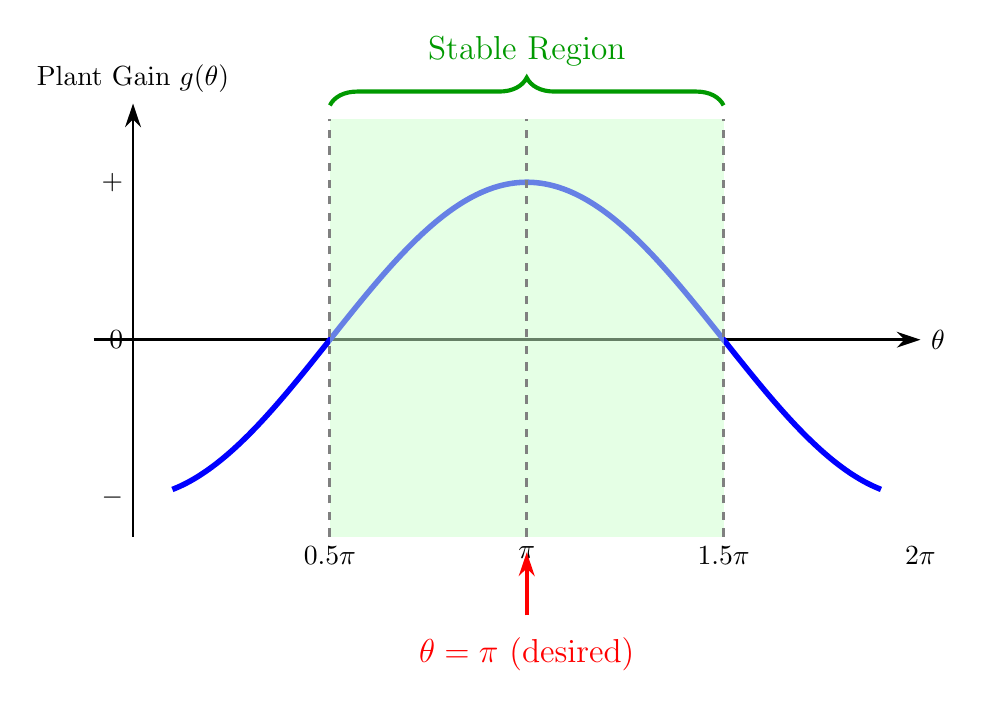
\begin{tikzpicture}[
    arrow/.style={-{Stealth[length=3mm, width=2mm]}, line width=1pt},
    label/.style={font=\large}
]
    % Axes
    \draw[arrow] (-0.5, 0) -- (10, 0) node[right] {$\theta$};
    \draw[arrow] (0, -2.5) -- (0, 3) node[above] {Plant Gain $g(\theta)$};
    
    % Labels on y-axis
    \node[left] at (0, 2) {$+$};
    \node[left] at (0, 0) {$0$};
    \node[left] at (0, -2) {$-$};
    
    % Plant gain curve (sinusoidal-like)
    \draw[line width=2pt, blue] plot[smooth, domain=0.5:9.5, samples=100] 
        (\x, {2*cos((\x-5)*36)});
    
    % Stable region shading
    \fill[green!20, opacity=0.5] (2.5, -2.5) rectangle (7.5, 2.8);
    
    % Stable region bracket
    \draw[decorate, decoration={brace, amplitude=10pt, raise=5pt}, line width=1.5pt, green!60!black]
        (2.5, 2.8) -- (7.5, 2.8) node[midway, above=15pt, font=\large, green!60!black] {Stable Region};
    
    % Vertical dashed lines
    \draw[dashed, gray, line width=1pt] (2.5, -2.5) -- (2.5, 2.8);
    \draw[dashed, gray, line width=1pt] (5, -2.5) -- (5, 2.8);
    \draw[dashed, gray, line width=1pt] (7.5, -2.5) -- (7.5, 2.8);
    
    % X-axis labels
    \node[below] at (2.5, -2.5) {$0.5\pi$};
    \node[below] at (5, -2.5) {$\pi$};
    \node[below] at (7.5, -2.5) {$1.5\pi$};
    \node[below] at (10, -2.5) {$2\pi$};
    
    % Desired operating point
    \draw[arrow, red, line width=1.5pt] (5, -3.5) -- (5, -2.7);
    \node[red, font=\large] at (5, -4) {$\theta = \pi$ (desired)};
    
\end{tikzpicture}
\caption{Plant gain $g(\theta)$ versus operating point $\theta$. The system is stable only within the shaded region.}
\end{figure}

\begin{itemize}
    \item If $|e| < 0.5\pi$: System remains stable
    \item If $|e| > 0.5\pi$: Plant gain changes sign $\rightarrow$ \textbf{Unstable!}
\end{itemize}

\subsection{Maximum Allowable Phase Error}

Using a safety margin:
\begin{equation}
|e|_{max} = 0.4\pi
\end{equation}

% =============================================================================
\section{Deriving Maximum Detectable Speed}
% =============================================================================

\subsection{From Phase Error Equation}

\begin{equation}
e_{ss} = \frac{2v\omega_n}{c \cdot \omega_{BW}} \leq 0.4\pi
\end{equation}

\subsection{Solve for Maximum Speed}

\begin{equation}
v_{max} = \frac{0.4\pi \cdot c \cdot \omega_{BW}}{2\omega_n} = \frac{\pi \omega_{BW}}{5\omega_n} \cdot c
\end{equation}

This is \textbf{equation (18)} in the paper:
\begin{equation}
\boxed{v_{max} = \frac{\pi \omega_{BW}}{5\omega_n} \cdot c \text{ (m/s)}}
\end{equation}

% =============================================================================
\section{Physical Interpretation}
% =============================================================================

\subsection{Analogy: Car Following}

% TikZ: Car Following Analogy
\begin{figure}[h]
\centering
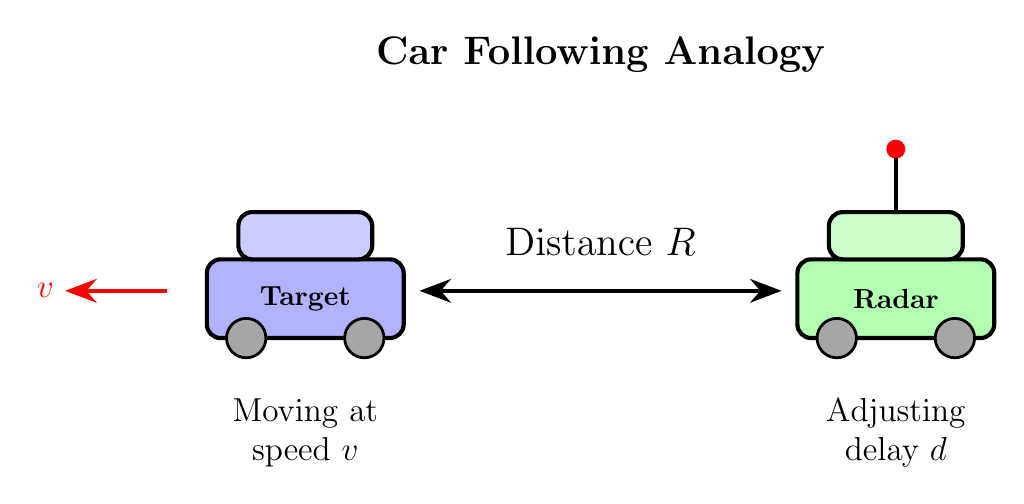
\begin{tikzpicture}[
    wheel/.style={circle, draw=black, fill=gray!70, minimum size=0.5cm, line width=1pt},
    carbody/.style={rectangle, draw=black, line width=1.5pt, rounded corners=5pt},
    arrow/.style={-{Stealth[length=4mm, width=3mm]}, line width=1.5pt},
    label/.style={font=\large}
]

    % Title
    \node[font=\Large\bfseries] at (5, 4) {Car Following Analogy};

    % === Target Car ===
    \begin{scope}[shift={(0,0)}]
        % Car body
        \draw[carbody, fill=blue!30] (0, 0.4) rectangle (2.5, 1.4);
        % Car top
        \draw[carbody, fill=blue!20] (0.4, 1.4) rectangle (2.1, 2);
        % Wheels
        \node[wheel] at (0.5, 0.4) {};
        \node[wheel] at (2.0, 0.4) {};
        % Label
        \node[font=\bfseries] at (1.25, 0.9) {Target};
    \end{scope}

    % Target label
    \node[label, align=center] at (1.25, -0.8) {Moving at\\speed $v$};

    % Velocity arrow
    \draw[arrow, red] (-0.5, 1) -- (-1.8, 1) node[left, font=\large] {$v$};

    % === Radar Car ===
    \begin{scope}[shift={(7.5,0)}]
        % Car body
        \draw[carbody, fill=green!30] (0, 0.4) rectangle (2.5, 1.4);
        % Car top
        \draw[carbody, fill=green!20] (0.4, 1.4) rectangle (2.1, 2);
        % Wheels
        \node[wheel] at (0.5, 0.4) {};
        \node[wheel] at (2.0, 0.4) {};
        % Label
        \node[font=\bfseries] at (1.25, 0.9) {Radar};
        % Antenna
        \draw[line width=1.5pt] (1.25, 2) -- (1.25, 2.8);
        \fill[red] (1.25, 2.8) circle (0.12);
    \end{scope}

    % Radar label
    \node[label, align=center] at (8.75, -0.8) {Adjusting\\delay $d$};

    % === Distance Arrow ===
    \draw[{Stealth[length=4mm, width=3mm]}-{Stealth[length=4mm, width=3mm]}, line width=1.5pt] 
        (2.7, 1) -- (7.3, 1) 
        node[midway, above=0.3cm, font=\Large] {Distance $R$};

\end{tikzpicture}
\caption{Car following analogy: The radar controller tries to ``follow'' the target by adjusting the delay $d$.}
\end{figure}

\begin{table}[h]
\centering
\renewcommand{\arraystretch}{1.5}
\begin{tabular}{ll}
\toprule
\textbf{Scenario} & \textbf{Result} \\
\midrule
Target moves slowly & Radar easily tracks \\
Target moves fast & Radar struggles to keep up \\
Target moves too fast & \textcolor{red}{Radar loses the target} \\
\bottomrule
\end{tabular}
\caption{Effect of target speed on radar tracking.}
\end{table}

\textbf{Maximum speed} = The fastest the target can move while radar still tracks it!

% =============================================================================
\section{Numerical Example}
% =============================================================================

From the paper's design:

\begin{table}[h]
\centering
\renewcommand{\arraystretch}{1.5}
\begin{tabular}{ll}
\toprule
\textbf{Parameter} & \textbf{Value} \\
\midrule
$\omega_{BW}$ & $2\pi \times 3820$ rad/s \\
$\omega_n$ & $2\pi \times 40000$ rad/s \\
$c$ & 340 m/s (sound in air) \\
\bottomrule
\end{tabular}
\caption{Design parameters from the paper.}
\end{table}

Calculation:
\begin{align}
v_{max} &= \frac{\pi \times 2\pi \times 3820}{5 \times 2\pi \times 40000} \times 340 \\
&= \frac{\pi \times 3820}{5 \times 40000} \times 340 \\
&= \frac{3.14159 \times 3820}{200000} \times 340 \\
&= \boxed{20.4 \text{ m/s}}
\end{align}

This is \textbf{much faster} than human chest movement ($\sim$0.04 m/s), so the radar works well!

% =============================================================================
\section{Speed vs Tracking Capability}
% =============================================================================

% TikZ: Speed Comparison Figure
\begin{figure}[h]
\centering
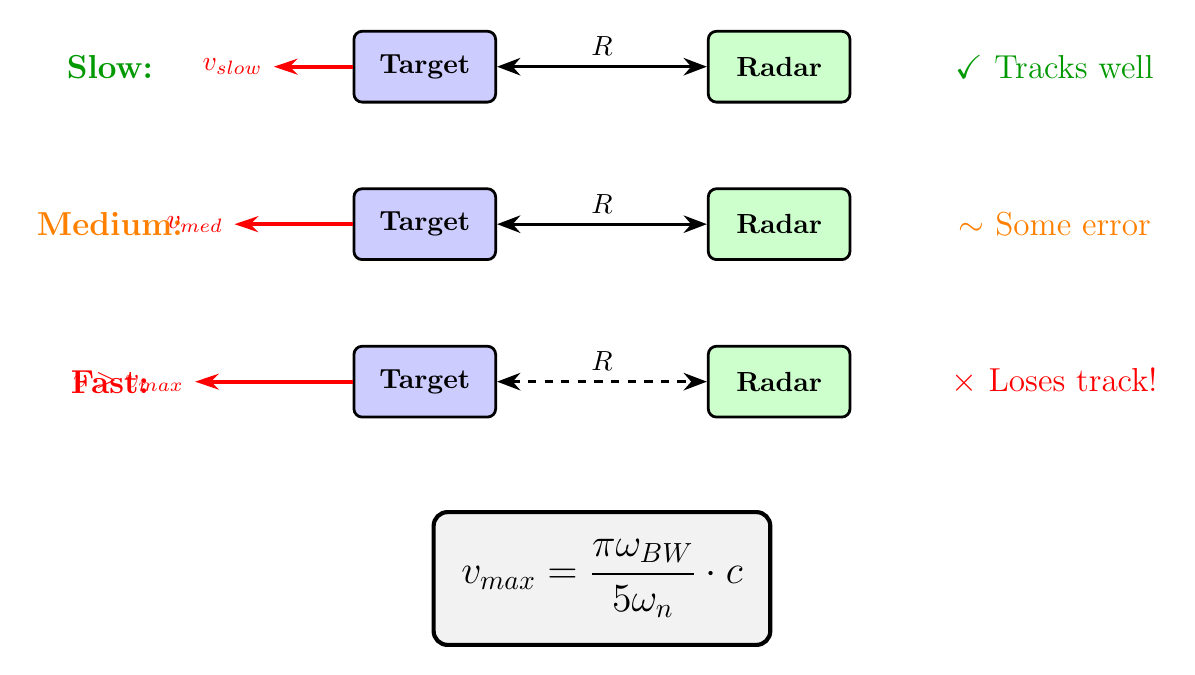
\begin{tikzpicture}[
    car/.style={rectangle, draw=black, line width=1pt, minimum width=1.8cm, 
                minimum height=0.9cm, rounded corners=3pt, font=\bfseries},
    arrow/.style={-{Stealth[length=3mm, width=2mm]}, line width=1.5pt},
    label/.style={font=\large\bfseries}
]

    % === Row 1: Slow Target ===
    \node[label, green!60!black] at (-2.5, 3) {Slow:};
    \node[car, fill=blue!20] (t1) at (1.5, 3) {Target};
    \node[car, fill=green!20] (r1) at (6, 3) {Radar};
    \draw[{Stealth}-{Stealth}, line width=1.2pt] (t1.east) -- (r1.west) 
        node[midway, above] {$R$};
    \draw[arrow, red] (t1.west) -- ++(-1, 0) node[left] {$v_{slow}$};
    \node[green!60!black, font=\large] at (9.5, 3) {$\checkmark$ Tracks well};

    % === Row 2: Medium Target ===
    \node[label, orange] at (-2.5, 1) {Medium:};
    \node[car, fill=blue!20] (t2) at (1.5, 1) {Target};
    \node[car, fill=green!20] (r2) at (6, 1) {Radar};
    \draw[{Stealth}-{Stealth}, line width=1.2pt] (t2.east) -- (r2.west) 
        node[midway, above] {$R$};
    \draw[arrow, red] (t2.west) -- ++(-1.5, 0) node[left] {$v_{med}$};
    \node[orange, font=\large] at (9.5, 1) {$\sim$ Some error};

    % === Row 3: Fast Target ===
    \node[label, red] at (-2.5, -1) {Fast:};
    \node[car, fill=blue!20] (t3) at (1.5, -1) {Target};
    \node[car, fill=green!20] (r3) at (6, -1) {Radar};
    \draw[{Stealth}-{Stealth}, line width=1.2pt, dashed] (t3.east) -- (r3.west) 
        node[midway, above] {$R$};
    \draw[arrow, red] (t3.west) -- ++(-2, 0) node[left] {$v > v_{max}$};
    \node[red, font=\large] at (9.5, -1) {$\times$ Loses track!};

    % Equation box
    \node[draw, fill=gray!10, rounded corners=5pt, line width=1.5pt, 
          font=\Large, inner sep=10pt] at (3.75, -3.5) 
        {$\displaystyle v_{max} = \frac{\pi \omega_{BW}}{5\omega_n} \cdot c$};

\end{tikzpicture}
\caption{Effect of target speed on radar tracking capability.}
\end{figure}

% =============================================================================
\section{Summary: Why Maximum Speed = Disturbance Rejection}
% =============================================================================

\begin{table}[h]
\centering
\renewcommand{\arraystretch}{1.8}
\begin{tabular}{ll}
\toprule
\textbf{Concept} & \textbf{Explanation} \\
\midrule
Disturbance & Doppler phase shift from target motion \\
Disturbance rate & Proportional to target speed $v$ \\
Controller job & Cancel phase shift by adjusting delay $d$ \\
Controller limit & Bandwidth $\omega_{BW}$ limits how fast it can respond \\
Failure mode & If target too fast $\rightarrow$ phase error too large $\rightarrow$ instability \\
Metric & $v_{max}$ = maximum speed before failure \\
\bottomrule
\end{tabular}
\caption{Summary of disturbance rejection concepts.}
\end{table}

\vspace{1cm}

% Final Key Equation Box
\begin{figure}[h]
\centering
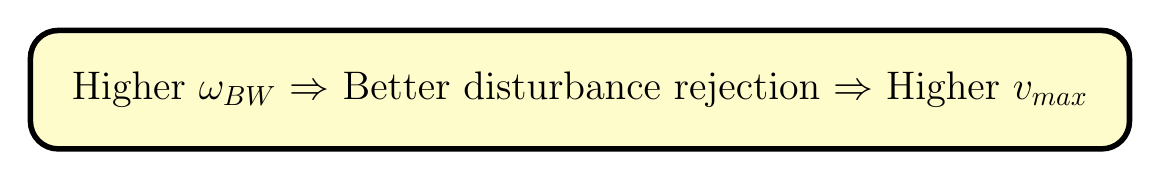
\begin{tikzpicture}
    \node[draw=black, fill=yellow!20, rounded corners=10pt, line width=2pt, 
          font=\Large, inner sep=15pt] at (0, 0) 
        {Higher $\omega_{BW}$ $\Rightarrow$ Better disturbance rejection $\Rightarrow$ Higher $v_{max}$};
\end{tikzpicture}
\end{figure}

\end{document}